\documentclass[british]{article}

\usepackage[british]{babel}% Recommended
\usepackage{csquotes}% Recommended

\usepackage[sorting=nyt,style=apa]{biblatex}

%\addbibresource{~/Tex/library.bib}
\addbibresource{C:/Users/Daniel/Documents/BibTex/library.bib}
\usepackage[margin=1in]{geometry}
\usepackage{booktabs}
\usepackage{amsmath}
\usepackage{graphicx}
\usepackage{listings}
\usepackage{enumerate}
\newcommand{\code}[1]{\texttt{#1}}
\newtheorem{defin}{Definition}
\newtheorem{prop}{Proposition}
\newtheorem{col}{Corollary}
\newtheorem{thm}{Theorem}
\usepackage{appendix}
\setlength{\parskip}{1em}
\usepackage{placeins}
\DeclareLanguageMapping{british}{british-apa}

\title{CS5014 - P1}
\author{170008773}
\date{\today}
\begin{document}
	\maketitle
	
	
	
	
	\section{Introduction}
	\label{intro}
	In this report we were asked to design and implement a regression model to predict energy consumption in resident houses. In this report we will mirror the work of \autocite{Candanedo2017} as closely as possible, in the time allowed, so we can compare results. Like \citeauthor{Candanedo2017} we  assume that it is desirable to better understand the impact different features have on energy consumption for prediction of other important phenomena, such as but not limited to ``determine[ing] adequate sizing of photovoltaics and energy storage to diminish power flow into the grid [and] to detect abnormal energy use patterns" \autocite{Candanedo2017}. Therefore we will develop several regression models that can tell us more about the impact certain features have on the overall energy usage. Here we will use three algorithms, each from a different class: Random forests (tree based) and Gradient Boosting (boosting based) and linear regression (coefficient based). Lastly we will mirror \citeauthor{Candanedo2017} in the use of the Mean Absolute Error (MAE) so that we can compare results. 
	
	\section{The learning pipeline}
	\label{content}
	
	\subsection{Cleaning the data}
	\label{cleaning}
	Since the data arrived relatively clean, this step in the process was fairly easy. After loading the data into a \code{pandas} data frame. The first thing we did was cast all columns to the correct type, namely \code{datetime} for the \code{date} column and \code{float} for all others. Secondly, we set the \code{date} column as the index to make use we could order the data correctly as desired. 
	
	\paragraph{Normalisation} Certain models, like the linear model can be sensitive to differences in scale between the features. This will become even more important when we start working on the feature elimination. Therefore we will normalise the data to the same scale, using a \code{MaxAbsScaler} from sci-kit-learn \autocite{Pedregosa2012}, before training and testing. We will do this for all the models to give them a fair comparison. It is also important to note that the test data is scaled according to the parameters of the training data since we don't want to give the model knowledge it's not supposed to have. 
	
	\paragraph{Cross Validation vs seperation} One choice is to use $k$-fold cross-validation or to separate the data into training and test data before hand. Initially we wanted to use cross-validation but we eventually decided that there was too little data for this. For cross-validation to be a useful metric we want to have low variance in our accuracy measures. To do this we should have a high $k$. This however would result in the folds becoming too small, meaning that we risk introducing (potentially different) biases into the testing phases. However if we choose a $k$ that is too small we take too much test data way from training, giving us a sub-realistic picture of the performance of our model, as well as increasing the variance of our end result. After concluding that there was no $k$ for which the result was both realistic and stable, we decided to divide the data into testing and training data before hand. We used 25\% of the data for testing and the rest for training, just like \citeauthor{Candanedo2017}. This seems to be an acceptable device according to the literature. 
	
	\subsection{Feature selection}
	\label{featureSelection}
	Since feature importance discovery is one of the main goals of this research we started out using all of the features. We deliberately chose models that allowed for some kind of automatic feature selection, based on their relative importance. After the models were trained we used their respective mechanisms to determine the most important features. We will discuss these mechanisms in more detail in section \ref{modelSelection}.
	
	\paragraph{Extraction} It is also worth noting that \citeauthor{Willmott2009} also had good success using extracted features. In particular, the extracted feature ``Seconds to midnight" (NSM) proved to be very influential. We did not have enough time however to pursue this avenue, beyond mirroring the work of  \autocite{Candanedo2017}, so we decided to leave this for future work. 
	
	\subsection{Selecting and training the model}
	\label{modelSelection}
	\paragraph{Models}Since it is our goal to gain a better understanding of how the various features impact the overall energy usage, it behoves us to pick models that can easily provide this information. A lot of regression models, like Neural Networks, do not provide this information natively. This would defeat a large part of the purpose of our research. After performing the experiments we will use the best performing model to carry out analysis of the features. 
	
	\subsubsection{Linear regression with recursive feature elimination} Although linear regression models do not natively provide mechanisms to eliminate features, this can still be achieved due to the simplicity of the model. Here we used the \code{RFE} module from sci-kit-learn. This module looks at the coefficients associated with each feature and recursively eliminates those with the smallest coefficients. 
	
	\subsubsection{Random Forests and gradient boosting} Random forests and Gradient boosting machines are ensemble methods \autocite{Breiman2001,Jeromeh1999}. One of their major advantages, and the main reasons we chose to use them, is that they provide native mechanisms to rank features in terms of importance. Due to this mechanism we could use the \code{feature\_selection.SelectFromModel} functionality form sci-kit-learn. In their respective papers, it is also claimed that they are robuster models, that can handle more diverse and dirtier data. This however, is less of a concern for us, since we cleaned and standardized the data before hand. 
	
	\subsection{Evaluating the model}
	\label{evaluation}
	
	\paragraph{Metrics}We must select a metric to judge our model by. Again we wanted to use a metric that was supported by our libraries, so this cut down the number of possibilities considerably. We also wanted a metric that would let us interpret the results easily since we are not just interested in raw performance, but in interpretability. This narrowed the possibilities down to the Root-Mean-Squared-Error  (RMSE) or the Mean-Absolute-Error (MAE). We eventually elected MAE since this provides a more neutral view of the accuracy \autocite{Willmott2009}.
	
	\paragraph{Evaluating the models} We ran all the models on the normalised training data and recorded their MAE on the test set. After that, we extracted the features in the manners discussed above and reran the models on the reduced feature set to see if this would increase the accuracy. After running all the models we selected the best performing model to use in our feature importance analysis. 
	
	\subsection{Discussing the results}
	\label{discussion}
	
	\begin{figure}[!ht]
		\begin{tabular}{|l|l|l|r|}
			\toprule
			{} &          Algorithm & Feature set &        MAE \\
			\midrule
			4 &     Random Forests &        full &  35.714633 \\
			5 &     Random Forests &     reduced &  36.488448 \\
			2 &  Gradient Boosting &        full &  48.186388 \\
			3 &  Gradient Boosting &     reduced &  49.125515 \\
			0 &             Linear &        full &  53.782201 \\
			1 &             Linear &     reduced &  53.979079 \\
			\bottomrule
		\end{tabular}
		\caption{Testing results for the various algorithms. Aranged in decending order of MAE}
		\label{resultsTable}
		
	\end{figure}
	Looking at figure \ref{resultsTable} we see that RF outperforms both GB and the linear model by a significant margin. It is also worth noting that both RF and linear perform worse on the reduced set, although none of the models gains a significant in-, or decreases in accuracy by switching between the full or reduced set. This leads us to conclude that the models are robust enough to deal with the less important variables after normalisation. 
	
	\paragraph{Feature importance} As stated at the beginning we will briefly examine the feature importance as indicated by the RF, since that model had the best accuracy. Looking at figure \ref{relImp} we see that the overall spread of the feature importance is low. In it's current configuration the RF will eliminate all features that are below the mean of all the importances. We can now see that it will eliminate quite a few features that still contribute a fair bit to the overall importance. It makes sense therefore, that our overall accuracy would go down. After eliminating we see that the features \code{lights, RH\_1, RH\_2, T3, RH\_3, RH\_5, T8, RH\_8, Press\_mm\_hg} and \code{ RH\_out} are deemed most important. This would suggest that it would be interesting to further investigate the impact of humidity on energy consumption. 
	
	\begin{figure}[!ht]
		\centering
		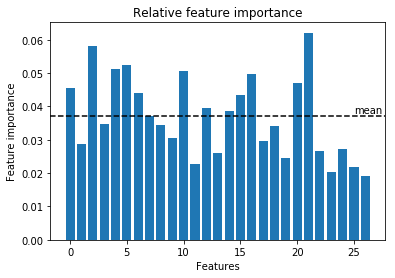
\includegraphics[width=0.5\textwidth]{relFeatureImp}
		\caption{Relative feature importance accoring to the Random Forest}
		\label{relImp}
	\end{figure}
	
	
	\subsection{limitations} This research has a number of limitations. Firstly there are limitations that are also present in \autocite{Candanedo2017}. Namely that the data was only collected from one house over a limited length of time. Therefore this runs a serious risk of introducing biases into the data and therefore into the conclusions. 
	
	Furthermore, it is also quite limited in it's scope. Ideally, we would have had more time to test more models on multiple metrics. We also did not research the effectiveness of possible extracted features. A line of research that proved quite useful for \citeauthor{Candanedo2017}. Lastly, we recognise that our analysis of both the data and the feature importance was extremely limited. 
	
	
	
	word count: 1315
	\printbibliography
\end{document}
